\documentclass[12pt]{article}
\usepackage{amsmath} 
\usepackage{amsthm} % Theorem Formatting
\usepackage{amssymb}    % Math symbols such as \mathbb
\usepackage{graphicx} % Allows for eps images
\graphicspath{ {images/} }
\usepackage[dvips,letterpaper,margin=1in,bottom=0.7in]{geometry}
\usepackage{tensor}
 % Sets margins and page size
\usepackage{amsmath}

\renewcommand{\labelenumi}{(\alph{enumi})} % Use letters for enumerate
% \DeclareMathOperator{\Sample}{Sample}
\let\vaccent=\v % rename builtin command \v{} to \vaccent{}
\usepackage{enumerate}
\renewcommand{\v}[1]{\ensuremath{\mathbf{#1}}} % for vectors
\newcommand{\gv}[1]{\ensuremath{\mbox{\boldmath$ #1 $}}}
% for vectors of Greek letters
\newcommand{\uv}[1]{\ensuremath{\mathbf{\hat{#1}}}} % for unit vector
\newcommand{\abs}[1]{\left| #1 \right|} % for absolute value
\newcommand{\avg}[1]{\left< #1 \right>} % for average
\let\underdot=\d % rename builtin command \d{} to \underdot{}
\renewcommand{\d}[2]{\frac{d #1}{d #2}} % for derivatives
\newcommand{\dd}[2]{\frac{d^2 #1}{d #2^2}} % for double derivatives
\newcommand{\pd}[2]{\frac{\partial #1}{\partial #2}}
% for partial derivatives
\newcommand{\pdd}[2]{\frac{\partial^2 #1}{\partial #2^2}}
% for double partial derivatives
\newcommand{\pdc}[3]{\left( \frac{\partial #1}{\partial #2}
 \right)_{#3}} % for thermodynamic partial derivatives
\newcommand{\ket}[1]{\left| #1 \right>} % for Dirac bras
\newcommand{\bra}[1]{\left< #1 \right|} % for Dirac kets
\newcommand{\braket}[2]{\left< #1 \vphantom{#2} \right|
 \left. #2 \vphantom{#1} \right>} % for Dirac brackets
\newcommand{\matrixel}[3]{\left< #1 \vphantom{#2#3} \right|
 #2 \left| #3 \vphantom{#1#2} \right>} % for Dirac matrix elements
\newcommand{\grad}[1]{\gv{\nabla} #1} % for gradient
\let\divsymb=\div % rename builtin command \div to \divsymb
\renewcommand{\div}[1]{\gv{\nabla} \cdot \v{#1}} % for divergence
\newcommand{\curl}[1]{\gv{\nabla} \times \v{#1}} % for curl
\let\baraccent=\= % rename builtin command \= to \baraccent
\renewcommand{\=}[1]{\stackrel{#1}{=}} % for putting numbers above =
\providecommand{\wave}[1]{\v{\tilde{#1}}}
\providecommand{\fr}{\frac}
\providecommand{\RR}{\mathbb{R}}
\providecommand{\NN}{\mathbb{N}}
\providecommand{\QQ}{\mathbb{Q}}
\providecommand{\seq}{\subseteq}
\providecommand{\e}{\epsilon}
\providecommand{\T}{\mathcal{T}}

\newtheorem{prop}{Proposition}
\newtheorem{thm}{Theorem}[section]
\newtheorem{axiom}{Axiom}[section]
\newtheorem{p}{Problem}[section]
\usepackage{cancel}
\newtheorem*{lem}{Lemma}
\theoremstyle{definition}
\newtheorem*{dfn}{Definition}
 \newenvironment{s}{%\small%
        \begin{trivlist} \item \textbf{Solution}. }{%
            \hspace*{\fill} $\blacksquare$\end{trivlist}}%
% ***********************************************************
% ********************** END HEADER *************************
% ***********************************************************

\begin{document}

{\noindent\Huge\bf  \\[0.5\baselineskip] {\fontfamily{cmr}\selectfont  %
Problem Set 1}         }\\[2\baselineskip] % Title
{ {\bf \fontfamily{cmr}\selectfont MATC27: Introduction to Topology}\\ {\textit{\fontfamily{cmr}%
\selectfont September 29, 2017, 1002678140}}}
{\large \textsc{Anmol Bhullar}} % Author name
\\[1.4\baselineskip]

\begin{p}
    Let $X = \{a,b,c,d\}$ where $a,b,c,d$ are pairwise disjoint. Define the topology
    $\mathcal{T} = \{\emptyset, X, \{c\}, \{a,b\}, \{c,d\}, \{a,b,c\}\}$ on $X$.
    \begin{enumerate}
        \item What are the open sets of $(X,\mathcal{T})$?
        \item What are the closed sets of $(X,\T)$?
        \item What are the clopen sets of $(X,\T)$?
    \end{enumerate}
    Make sure to provide justification for your answers.
\end{p}
\begin{s}
    (a) On page 76 of Munkres' Topology, it is stated that for a set $U\subseteq X$ (where $(X,\T)$ is a topological space) to be open, 
    $U$ has to belong to the collection $\T$. Thus, if we want to know the open sets of $(X,\T)$, we can simply look at the members
    of $\T$. Note, that $\T$ is a (small) finite set so this is possible via simple observation. Therefore, the open sets of $(X,\T)$ are as follows:
    \[ \emptyset,\: X,\: \{c\},\: \{a,b\},\: \{c,d\},\: \{a,b,c\} \]
    (b) On page 93 of Munkres' Topology, it is stated that a set $U\subseteq X$ (where $(X,\T)$ is a topological space) is closed if the
    set $X - U$ (i.e. $U^{c}$) is open. Thus, to get a list of all the closed sets in $(X,\T)$, 
    we can consider every possible subset of $X$ and check whether the complement of that subset is a member of $\T$. This is how 
    we obtain the following list of closed sets in $(X,\T)$:
    \[ \emptyset,\: X,\: \{d\},\: \{a,b\},\: \{c,d\},\: \{a,b,d\} \]
    (c) A set $U\subseteq X$ (where $(X,\T)$ is a topological space) is said to be clopen if it is both open and closed. Thus, to get
    a list of all the clopen sets of $(X,\T)$, we can take the intersection of the set of all open sets and the set of all closed sets.
    We computed these sets in (a) and (b). Thus, we see that the clopen sets in $(X,\T)$ are:
    \[ \emptyset,\: X,\: \{a,b\},\: \{c,d\} \]
\end{s}

\newpage
\begin{p}
    Let $X$ be a topological space. Prove that:
    \begin{enumerate}
        \item $\emptyset$ and $X$ are closed.
        \item Arbitrary intersection of closed sets in $X$ are closed in $X$
        \item Finite unions of closed sets in $X$ are closed in $X$
    \end{enumerate}
\end{p}
\begin{s}
    (a) Consider the definition of a topology on page 76 in Munkres' Topology. By axiom 1, we have that a topology $\T$ (on $X$) will
    always contain $\emptyset$ and $X$. By the definition of an open set (on the same page), we have that both
    $\emptyset$ and $X$ are open in $(X,\T)$.
    By the definition of a closed set (on page 93), we have that $\emptyset,\:X$ are also
    closed if their complements are contained in $\T$. Thus, note that:
    \[ (\emptyset)^{c} = X\in\T \qquad (X)^{c} = \emptyset\in\T\qquad(\text{containment given by axiom 1}) \]
    which implies that both $X$ and $\emptyset$ are also closed as wanted. \\

    (b) Let $(X,\T)$ be a topological space and $\{Y_i\}$ (where $i\in I$ is the index set) be a family of subsets of $X$. Then recall the DeMorgan Laws:
    \begin{align}
        \bigcup_{i\in I}\: (X\:\backslash\: Y_i) = X\:\backslash\:\bigg{(}\bigcap_{i\in I} Y_i\bigg{)} \\ \bigcap_{i\in I}\: (X\:\backslash\: Y_i) = X\:\backslash\:
        \bigg{(}\bigcup_{i\in I} Y_i\bigg{)}
    \end{align}
    First, note if $\{Y_i\}$ is a collection of closed sets in $(X,\T)$ which is indexed by $I$, then $\cap_{i\in I}\:Y_i$ is the intersection of an arbitrary collection
    of closed sets. Using this, we want to show $\cap_{i\in I}\: Y_i$ is closed or equivalently, via the definition of a closed set, we can show that:
    \[ X\:\backslash\:\bigg{(}\bigcap_{i\in I} Y_i\bigg{)} \quad \text{is open} \]
    Then, by the DeMorgan Laws (specifically (1)), we have that:
    \[ X\:\backslash\:\bigg{(}\bigcap_{i\in I} Y_i\bigg{)} = \bigcup_{i\in I}\:(X\:\backslash\:Y_i) \]
    Since, $\{Y_i\}$ is a collection of closed sets in $(X,\T)$, then for any $i\in I$, it holds $X\:\backslash\:Y_i$ is open. By axiom 2 of
    a topology (page 76), we know that arbitrary unions of open sets are open. Thus $\cup_{i\in I}\: (X\:\backslash\: Y_i)$ is open,
    immediately implying that $X\backslash(\cap_{i\in I}\: Y_i)$ is open. Therefore by definition of a closed set, $\cap_{i\in I}\: Y_i$ is closed. \\

    (c) For $k\in\NN$, $0<i\leq k$, let $\{Y_i\}$ be a finite collection of closed sets in $(X,\T)$. We want to show $\cup_{i=1}^k\:  Y_i$
    is closed. This can be done by considering (2) which gives us the equality:
    \[ X\:\backslash\:\bigg{(}\bigcup_{i=1}^k\:Y_i\bigg{)} = \bigcap_{i=1}^k\: (X\:\backslash\:Y_i) \]
    Since $Y_i$ is closed for every $i$, $X\backslash Y_i$ is then open. Then by axiom 3 of a topology (page 76), it follows that,
    $\cap_{i=1}^k\: (X\:\backslash\:Y_i)$ is open since the intersection is only of a finite number of open sets. Thus, $X\backslash(\cup_{i=1}^k Y_i)$ is
    open which implies $\cup_{i=1}^k Y_i$ is closed.
\end{s}

\newpage

\begin{p}
    Consider the nine topologies on the set $X = \{a,b,c\}$ indicated in Figure 12.1 or Example 1 of $\S 12$. Compare
    them; that is, for each pair of topologies, determine whether they are comparable, and if so, which is
    the finer. 

    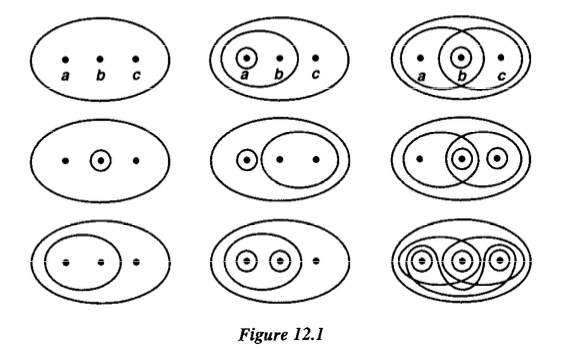
\includegraphics[width=\textwidth]{figure12-1}
\end{p}
\begin{s}
    First, let us write out the topologies listed in the figure above (list written in order left to right then moving to the leftmost set of the row underneath)
    \begin{align*}
        \T_1 = \{\emptyset, X\} && \T_2 = \{\emptyset, \{a\}, \{a,b\}, X\} && \T_3 = \{\emptyset,\{a,b\},\{b\},\{b,c\},X\} \\
        \T_4 = \{\emptyset, \{b\}, X\} && \T_5 = \{\emptyset, \{a\}, \{b,c\}, X\} && \T_6 = \{\emptyset,\{a,b\},\{b\},\{c\},\{b,c\},X\} \\
        \T_7 = \{\emptyset, \{a,b\}, X\} && \T_8 = \{\emptyset, \{a\},\{b\},\{a,b\},X\} &&
        \T_9 = \{\emptyset, \{a\},\{b\},\{c\}, \{a,b\}, \{b,c\}, \{a,c\}, X\}
    \end{align*}
    Let $i\in\{1,\hdots,9\}$. We immediately see that $\T_1$ is a subset of every other $\T_i$ and $\T_9$ is the super set of every
    other $\T_i$. Thus, $\T_1$ is coarser than every other topology and $\T_9$ is finer than every other topology. Via more 
    observation, we see that $\T_2$, $\T_3$, $\T_6$, $\T_8$ are finer than $\T_7$. Moreover, $\T_3$, $\T_6$, $\T_8$ are finer than $\T_4$.
    $\T_8$ is finer than $\T_2$. $\T_6$ is finer than $\T_3$. Finally, the following pairs of topologies are incomparable:
    \[ (\T_2, \T_5),\quad (\T_5,\T_8),\quad (\T_3,\T_8),\quad (\T_2,\T_3) \quad (\T_6, \T_8)\]
\end{s}

\newpage
\begin{p}
    Show that the collection $\T_C$ given in Example 4 of $\S 12$ is a topology on the set $X$. Is the collection
    \[ \T_{\infty} = \{U : X - U\:\text{is infinite or empty or all of}\:X\} \]
    a topology on $X$?
\end{p}
\begin{s}
    First, we show that $\T_C$ is a topology.

    Choose $U = X$, then $X - X = \emptyset$ which is certainly countable. Thus $X \in \T_C$.
    Choose $U = \emptyset$, then $X - \emptyset = X$ which is certainly equal to $X$. Then $\emptyset\in \T_C$.
    Thus, condition 1 for $\T_C$ to be a topology is fulfilled. Now, we show that the unions of arbitrary elements of $\T_C$
    are in $\T_C$. Let $\{U_i\}$ $(i\in I$ index set$)$ be an arbitrary collection of elements of $\T_C$. We want to show $\cup\:U_i\in\T_C$.
    Consider one of the DeMorgan laws:
    \begin{align*}
        % U_j \subseteq \bigcup_i U_i \implies (\bigcup_i U_i)^c \subseteq (U_j)^c \\
        \big{(}\bigcup U_i\big{)}^c = \bigcap\: (U_i)^c
    \end{align*}
    Then, note that $U_i\in\T_C$ so $(U_i)^c$ is either countable or all of $X$. First consider, the case that for all $i\in I$, $(U_i)^c = X$, then
    the intersection of such $(U_i)^c$ simply produces $X$ so that $\cup\: U_i = \emptyset \in \T_C$. Now, suppose there is at least one $i\in I$ such that $(U_i)^c \neq X$.
    Then, in the intersection of such a collection, we can safely ignore all such elements equal to $X$ since they are not the smallest set in the collection.
    Thus, we can assume that for no $i\in I$, $(U_i)^c = X$ so we have that $(U_i)^c$ is countable. Note that for any $j\in I$, we have that
    $\cap\:(U_i)^c \subseteq (U_j)^c$ and since $U_j\in\T_C$, we have that $(U_j)^c$ is countable so that $\cap\:(U_i)^c$ is also countable.
    This implies that $\cup\:U_i\in\T_C$ as wanted. Now, we want to show that intersections of a finite number
    of elements of $\T_C$ are in $\T_C$ i.e. if $\{U_i\}$ is a finite collection of elements of $\T_C$ (so $I$ is a finite index set), then $\cap\: U_i \in \T_C$.
    Note that:
    \[ \big{(}\bigcap U_i\big{)}^c = \bigcup \big{(}U_i\big{)}^c \qquad (\text{DeMorgan's Law})\]
    Choose $U_j\in\T_C$, then either $(U_j)^c$ is countable or equal to $X$. Suppose \textit{at least one} $j\in I$ has the property that $(U_j)^c = X$, then
    $\cup\:(U_j)^c = X \in \T_C$ as wanted. Therefore, suppose no such $j\in I$ exist with that property. Then for any $j\in I$, we have that $(U_j)^c \neq X$, 
    thus, $(U_j)^c$ is countable, and we know that
    the union of a finite number of sets is still a countable set. Therefore $(\cap\:U_i)^c$ is countable, which implies that
    $\cap\: U_i \in \T_C$ thus fulfilling axiom 3 for a topology. Since, we have shown that $\T_C$ fulfills all three axioms that are required to be a topology, 
    we have that $\T_C$ is a topology. \\

    Now, we show that $\T_{\infty}$ is not a topology. Let $\T_{\infty}$ be a topology on $X = \RR$. Then the set:
    \[ \{[-i,-i-1]\subset\RR: i\in\NN\} \]
    is a collection of sets of $\RR$ whose complements are infinite sets in $\RR$. Similarly, $\{[i,i+1]:i\in\NN\}$ is also
    a collection of sets of $\RR$ whose complements are infinite sets in $\RR$. Then, the union of the elements in both of
    these collections is a union of arbitrary elements of $\T_{\infty}$ so the formed set should also be in $\T_{\infty}$ but note:
    \[ \bigcup_{i\in\NN} ([-i,i-1] \cup [i,i+1]) = (-\infty, 1] \cup [1,\infty) \] 
    the complement of this set is equal to $(-1,1)$ which is not equal to $\RR$ and is not infinite in $\RR$. This breaks axiom 2 of a topology, implying that
    $\T_{\infty}$ is not a topology.
\end{s}

\newpage
\begin{p}
    Let $\{\T_{\alpha}\}$ be a family of topologies on $X$.
    \begin{enumerate}
        \item Show $\cap\T_{\alpha}$ is a topology on $X$. Is $\cup\T_{\alpha}$ a topology on $X$?
        \item Show that there is a unique smallest topology on $X$ containing all the collections $\T_{\alpha}$, and
            a unique largest topology contained in all $\T_{\alpha}$.
        \item If $X = \{a,b,c\}$, let
            \[ \T_1 = \{\emptyset, X, \{a\}, \{a,b\}\}\qquad\text{and}\qquad\T_2 = \{\emptyset,X,\{a\},\{b,c\}\} \]
            Find the smallest topology containing $\T_1$ and $\T_2$, and the largest topology contained in $\T_1$ and $\T_2$.
    \end{enumerate}
\end{p}
\begin{s}
    (a) Let $A$ be the indexing set for the collection $\{T_{\alpha}\}$. Note that since $\T_{\alpha}$ is a topology
    for every $\alpha\in A$, it follows that $\emptyset \in \cap \T_{\alpha}$ and $X\in \cap\T_{\alpha}$. Now, let $\{U_i\}$
    (with index set $i\in I$) be a collection of arbitrary elements of the set $\cap\T_{\alpha}$. We show that 
    $\cup\: U_i \in \cap \T_{\alpha}$. Note, that $\{U_i\}\subseteq\cap\:\T_{\alpha}$, so $\{U_i\}\subseteq\T_{\alpha}$
    for arbitrary $\alpha\in A$. This implies that $\cup\:U_i\in\T_{\alpha}$ (axiom 2 of a topology). Since our choice 
    of $\T_{\alpha}$ was arbitrary, this holds for every $\alpha\in A$ so we have that $\cup\:U_i\in\cap\:\T_{\alpha}$. It is left
    to show that for a finite collection $\{U_i\}$ ($i\in I$ a finite indexing set) of elements of $\cap\:\T_{\alpha}$, we have:
    $\cap\:U_i\in\cap\:\T_{\alpha}$. Note that, since $\T_{\alpha}$ is a topology for an arbitrary $\alpha\in A$, it follows
    that $\cap\:U_i\in\T_{\alpha}$ (axiom 3 of a topology). Since our
    choice of $\T_{\alpha}$ was arbitrary, this result holds for every $\alpha\in A$ so $\cap\:U_i \in \cap\: \T_{\alpha}$.
    Thus, $\cap\:\T_{\alpha}$ is a topology on $X$ since it fulfills all 3 axioms for a set to be a topology. \\
    It is left to show that the union of a collection of topologies is not necessairly a topology.
    Let us define $\T_1$ and $\T_2$ the same way they are defined in 5(c). The union of $\T_1$ and $\T_2$ produces the set
    $\{\emptyset, X, \{a\}, \{a,b\}, \{b,c\}\}$ but consider $\{a,b\}\cap\{b,c\}\not\in(\T_1\cup\T_2)$ breaking axiom 3 of a topology.

    (b) Claim: $\cap\:\T_{\alpha}$ is the unique largest topology contained in all of $\T_{\alpha}$. By 5(a), we know that
    $\cap\:\T_{\alpha}$ is a topology. So, now we prove that $\cap\:\T_{\alpha}$ is the largest topology contained
    in $\{\T_{\alpha}\}$. We prove this via contradiction so, assume there exists a topology $\T_1$ such that
    $\T_1$ is contained in all of $\T_{\alpha}$ and $\cap\:T_{\alpha} \subset \T_1$. Then, there exists
    $U\in\T_1$ such that $U\not\in\cap\:\T_{\alpha}$. Since $U\not\in\cap\:\T_{\alpha}$, then there exists $\beta\in A$
    such that $U\not\in\T_{\beta}$. But this implies that $\T_1$ is not contained in all of $\T_{\alpha}$ which is a contradiction.
    Thus, $\T_1$ cannot exist, so $\cap\:\T_{\alpha}$ is the largest topology contained in all of $\T_{\alpha}$. Finally,
    uniqueness of $\cap\:\T_{\alpha}$ is left to prove. Assume it is not unique i.e. there exists $\T_2$ such that
    $\T_2$ and $\cap\:\T_{\alpha}$ are the largest topologies contained in all of $\T_{\alpha}$ but $\T_2\neq\cap\:\T_{\alpha}$.
    Since $\T_2\neq\cap\:\T_{\alpha}$, then there exists $U\in\T_2$ but $U\not\in\cap\:\T_{\alpha}$, 
    but if $U\not\in\cap\:\T_{\alpha}$, then there exists $\beta\in A$ such that $U\not\in\T_{\beta}$ which is a contradiction.
    Thus, by $\T_2$ cannot exist (since that was our assumption). So $\cap\:\T_{\alpha}$ is the unique largest topology
    contained in all of $\T_{\alpha}$.\\
    Claim: The smallest topology $\T$ containing every $\T_{\alpha}$ is given by:
    \begin{align}
        \T = \bigcap_{i\in I}\: \{\T_i\:\text{is a topology}: \T_{\alpha} \subseteq \T_i\:\text{for every}\:\alpha\in A\} 
    \end{align}
    Since $\T$ is the intersection of a collection of topologies, by (a), we have that $\T$ is actually a topology. Now, we
    prove that it is the smallest topology containing every $\T_{\alpha}$. Suppose that it is not. Then, there exists a topology
    $\T_1$ such that $\T_1\subset\T$ and for every $\alpha\in A$, $\T_{\alpha}\subseteq\T_1$. Note, that by definition of the set
    in (3) above, we have that $\T_1\in\{\T_i\}$, thus it is impossible that $\T_1 \subset \T$ which is a contradiction to our
    assumption $\T_1 \subset \T$, thus $\T_1$ cannot exist and $\T$ is the smallest topology containing every $\T_{\alpha}$. By
    a similar argument, it also follows that $\T$ is unique.
    \\

    (c) Claim: The smallest topology containing $\T_1$ and $\T_2$ is 
    \[ \T_3 := \{\emptyset, X, \{a\}, \{a,b\}, \{b,c\}, \{b\} \}  \]
    To show that $\T_3$ is the smallest topology that contains $\T_1$ and $\T_2$, assume that it is not and there exists
    $\T^{'}$ s.t. it contains $\T_1$ and $\T_2$ and $\T^{'}\subset\T_3$. Then, $\exists\:x\in\T_3$ s.t. $x\not\in\T^{'}$.
    We immediately know that $x$ cannot be any element that is in $\T_1$ and $\T_2$, because otherwise $\T^{'}$ would
    not contain $\T_1$ or $\T_2$. However, the only element that is in $\T_3$ that is not already in $\T_1$ or $\T_2$
    is the singleton $\{b\}$. So, $\T^{'} = \T_3 - \{b\}$, which implies that:
    \[ \T^{'} = \{\emptyset, X, \{a\}, \{a,b\}, \{b,c\} \} \]
    but this is not a topology since the intersection of the finite collection $\{\{a,b\},\{b,c\}\}$ of elements
    of $\T^{'}$ is not in $\T^{'}$. Thus, $\T^{'}$ cannot exist and the smallest topology containing $\T_1$ and $\T_2$
    is $\T_3$. It is left to find the largest topology contained in $\T_1$ and $\T_2$. Claim: $\T_4$ is the largest
    topology contained in $\T_1$ and $\T_2$ where:
    \[ \T_4 := \{\emptyset, X, \{a\}\} \]
    This follows from 5(b) and the fact that $\T_4 = \T_1 \cap \T_2$.
\end{s}

\begin{p}
    Show that if $\mathcal{A}$ is a basis for a topology on $X$, then the topology generated by $\mathcal{A}$ equals the intersection
    of all topologies of all topologies on $X$ that contain $\mathcal{A}$. Prove the same if $\mathcal{A}$ is a subbasis.
\end{p}
\begin{s}
    Case 1: $\mathcal{A}$ is a basis. Let $\T$ be the basis generated by $\mathcal{A}$ and let $\{\T_{\alpha}\}$ be the collection
    of topologies that contains $\mathcal{A}$ ($\alpha\in A$ is the indexing set). Then showing that $\T = \cap\:\T_{\alpha}$ is
    equivalent to showing that $\T$ is the coarsest topology in $\{\T_{\alpha}\}$. This follows from the fact that since
    $\mathcal{A}$ generates $\T$, then $\mathcal{A}\subset\T$ so $\T\in\{\T_{\alpha}\}$. \\

    To prove $\T$ is the coarsest topology in $\{\T_{\alpha}\}$ assume that $\T$ is not the coarsest topology that contains $\mathcal{A}$. 
    Then, there exists a topology $\T_1$ such that
    $\T_1\subset\T$ and $\T_1\in\{\T_{\alpha}\}$. Since $\T_1\subset\T$, there exists $U\in\T$ such that $U\not\in\T_1$. Since
    $\T$ is generated by $\mathcal{A}$, we have that:
    \[ \forall\:x\in U,\:\exists\:B\in\mathcal{A}\:\:\text{such that}\:\:x\in B\subset U \]
    Denote such sets of $B$, by $\{B_x\}$. Since $\mathcal{A}\subset\T_1$, then $B_x\in\T_1$ for all $x\in U$. However,
    since $\T_1$ is a topology, $\cup\:B_x \in \T_1$ but $\cup\:B_x = U \not\in \T_1$. This is a contradiction which implies
    that $\T_1$ cannot exist. Thus, there is no topology smaller than $\T$ such that $\mathcal{A}\subset\T$ which implies that
    $\T = \cap\:\T_{\alpha}$ as wanted. \\

    Case 2: $\mathcal{A}$ is a subbasis. Then via the definition of a subbasis, we have that: given any $U\in\T$, we have 
    that there exists finite sets $U_1,\hdots,U_k$ in $\mathcal{A}$ such that the $\cap_{i=1}^k U_i = U$. Again, as in the previous
    case, rather than show $\T = \cap\:\T_{\alpha}$, we will instead show that $\T$ (i.e. the topology generated by $\mathcal{A}$) is
    the smallest topology that contains $\mathcal{A}$. We prove this via contradiction so suppose $\T$ is not the smallest topology containing $\mathcal{A}$. Then,
    there exists a topology $\T_1 \subset \T$ such that $\mathcal{A}\subseteq\T_1$. Since $\T_1\subset\T$, then there exists
    $U\in\T$ such that $U\not\in\T_{\alpha}$. Furthermore, by definition of $\mathcal{A}$ (and that $\T$ is generated by $\mathcal{A}$),
    there exists elements $U_1,\hdots,U_k\in\mathcal{A}$ such that $\cap_{i=1}^k U_i = U\in\T$. But since $\mathcal{A}\subseteq\T_1$, we
    have that $U_1,\hdots,U_k\in\T_1$. Since this is a finite collection of elements of $\T_1$, the intersection between this finite
    collection must also be in $\T_1$. But this is a contradiction because by our assumption $U\not\in\T_1$. Thus, $\T_1$ cannot exist
    so $\T$ is the smallest topology that contains $\mathcal{A}$. Therefore $\T = \cap\: \{\T_{\alpha}: \mathcal{A}\subseteq\T_{\alpha}\}$ as wanted.
\end{s}

\begin{p}
    Prove that $\mathcal{B} = \{(a,b)\times(c,d):a,b,c,d\in\QQ, a<b,c<d\}$ is a basis for $\RR^2$.
\end{p}
\begin{s}
    In order to show $\mathcal{B}\subseteq\RR^2$ is a basis, we first prove the first condition. Thus, we want to show that
    if $x\in X$, then there is at least one basis element $B\in\mathcal{B}$ containing $x$. To do this, let $fl$ and $cl$
    be the floor and ceiling functions respectively. Then choose an arbitrary $x=(x_1,x_2)\in\RR^2$. Note, that by
    definition of the floor and ceiling functions, $fl(x_1-1) < x < cl(x_1+1)$ and additonally, $fl(x_1-1)\in\mathbb{Z}\subset\QQ$
    and $cl(x_1+1)\in\mathbb{Z}\subset\QQ$ so we have that:
    \[ x\in (fl(x_1-1),cl(x_1+1))\times(fl(x_2-1),cl(x_2+1))\in\mathcal{B}\]
    Now, we need to prove that if $x\in\RR^2$ belongs to the intersection of two basis elements $B_1$ and
    $B_2$ (of $\mathcal{B}$), then there is a basis element $B_3$ containing $x$ such that $B_3\subseteq B_1\cap B_2$.
    So, let us define:
    \begin{align*}
        B_1 &= \{(a_1,a_2)\times(b_1,b_2):a_1,a_2,b_1,b_2\in\QQ, a_1<a_2,b_1<b_2\} \\
        B_2 &= \{(a_3,a_4)\times(b_3,b_4):a_3,a_4,b_3,b_4\in\QQ, a_3<a_4,b_3<b_4\}
    \end{align*}
    Let $x = (x_1,x_2)$. If $x\in B_1\cap B_2$, then by the definition of cross product, we have that:
    \[ x_1\in (a_1,a_2)\cap(a_3,a_4)\neq\emptyset \qquad x_2\in(b_1,b_2)\cap(b_3,b_4)\neq\emptyset \]
    and, we also obtain (def'n of intersection) that:
    \[ x_1 \in (a_1,a_2) \implies x_1 > a_1 \qquad x_1\in (a_3,a_4) \implies a_4 > x_1 \]
    Choose rational $\epsilon_1$ such that $a_1 < \epsilon_1 < x_1$. This can be done since the rationals are dense within $\RR$ i.e. between two
    reals ($a_1$ and $x$), there exists a rational number. Repeat a similar process to obtain a rational $x_1 < \epsilon_2 < a_4$. Then:
    \begin{align}
        x_1 \in (\epsilon_1,\epsilon_2) \subset (a_1,a_2)\cap(a_3,a_4)
    \end{align}
    We can repeat a similar process on $x_2$ to
    obtain two additional rational numbers $\epsilon_3$ and $\epsilon_4$ such that 
    \begin{align}
        x_2\in(\epsilon_3,\epsilon_4)\subset(b_1,b_2)\cap(b_3,b_4)
    \end{align}
    Since $\epsilon_1,\epsilon_2,\epsilon_3,\epsilon_4\in\QQ$, we have that 
    $(\epsilon_1,\epsilon_2)\times(\epsilon_3,\epsilon_4)\in\mathcal{B}$. Combining (4) and (5), we have that:
    \[ x = (x_1,x_2) \in (\epsilon_1,\epsilon_2)\times(\epsilon_3,\epsilon_4)\subset B_1\cap B_2 \]
    as wanted. Thus $\mathcal{B}$ is a basis.
\end{s}

\newpage

\begin{p}
    Let $X = \mathbb{R}$ equipped with the topology $\T = \{\emptyset, \RR\} \cup \{(x,\infty):x\in\RR\}$. Is $\T$ comparable
    with the standard topology $\T_{\text{std}}$, and if so, which one is finer?
\end{p}
\begin{s}
    Recall that $\T_{\text{std}} = \{(a,b)\subset\RR: a,b\in\RR, a<b\}$. Claim: $\T_{\text{std}}$ is finer than $\T$ i.e. 
    $\T \subseteq \T_{\text{std}}$. Thus, all we need to show is that for all $U\in\T$, $U\in\T_{\text{std}}$. So assume
    $U\in\T$. Then, if $U = \emptyset$ or $U = \RR$, then it automatically follows $U\in\T_{\text{std}}$ since both are
    topologies on $\RR$. Thus, assume $U\not\in\{\emptyset,\RR\}$, which implies that $U = (x,\infty)$ for arbitrary $x\in\RR$.
    Consider the collection of elements of $\T_{\text{std}}$:
    \[ \mathcal{C} = \{(x,x+1),(x,x+2),(x,x+3),\hdots\} = \{(x,x+i)\subset\RR: i\in\NN\} = \{U_i\}_{i\in\NN}\]
    Since $\mathcal{C}\subset\T_{\text{std}}$, then $\cup\:U_i \in \T_{\text{std}}$. Furthermore, note that
    $U = (x,\infty) = \cup\:U_i$. Thus, we have that for an arbitrary element $U\in\T$, $U\in\T_{\text{std}}$ which
    implies that $\T\subset\T_{\text{std}}$ so that $\T_{\text{std}}$ is finer than $\T$. Furthermore, since we know
    that open sets in $\T$ are of the form $(x,\infty)$ (the ones that aren't equal to $\emptyset$ or $\RR$ that is),
    we obtain that $(0,1)\not\in\T$ but $(0,1)\in\T_{\text{std}}$ so we obtain the result that $\T_{\text{std}}$ is \textit{strictly} finer
    than $\T$.
\end{s}

\end{document}
